\section{最优解的敏感性}
\label{sec:opt-smooth-sensitivity}

上一节固定问题，研究算法返回的点离真正的最优解有多远。但目标中的数据往往来自测量或估计，本身就有误差。即使算法把手中的问题解得完全精确，所得的也只是“带误差数据的问题”的最优解。本节改变目标中的数据或参数，比较各个问题被精确求解后的最优解，判断问题本身对数据是否敏感。这是问题的性质，与用什么算法无关。

\subsection{扰动问题与解映射}
\label{sec:opt-smooth-solution-map}

\paragraph{一族问题}
设参数$\bm b$取值于某个集合，对每个$\bm b$给定$\mathbb R^d$上的可微目标$f_{\bm b}$。每个$\bm b$对应一个不同的无约束优化问题$\min_{\bm x}f_{\bm b}(\bm x)$，记其最优解集为$S(\bm b)=\argmin_{\bm x}f_{\bm b}(\bm x)$。映射$\bm b\mapsto S(\bm b)$称为\term{解映射}（solution map）。研究敏感性，就是比较$S(\bm b)$与$S(\bm c)$：两个不同问题的精确最优解。这与上一节的比较对象不同，那里比较的是同一个问题上的理想迭代与实际迭代，两者都还没有收敛到最优解。

\paragraph{三种误差的区分}
以二次目标族$f_{\bm b}(\bm x)=\tfrac12\bm x^\top\bm H\bm x-\bm b^\top\bm x$为例，$\bm H\succ\bm0$，唯一解为$\bm x_{\bm b}=\bm H^{-1}\bm b$。设真实数据是$\bm b$，手中只有带误差的$\bm b+\delta\bm b$，算法在后者上返回$\tilde{\bm x}$。三角不等式把总误差拆成两部分：
\[
  \lVert\tilde{\bm x}-\bm x_{\bm b}\rVert_2\leq\underbrace{\lVert\tilde{\bm x}-\bm x_{\bm b+\delta\bm b}\rVert_2}_{\text{算法求解误差}}+\underbrace{\lVert\bm x_{\bm b+\delta\bm b}-\bm x_{\bm b}\rVert_2}_{\text{数据误差引起的解变化}} .
\]
第一项可以通过多迭代几步缩小；第二项只取决于问题，算法再精确也去不掉。取$\bm H=\operatorname{diag}(1,0.1)$、$\bm b=(1,0.1)^\top$，解为$(1,1)^\top$；若$b_2$测成$0.2$，误差只有$0.1$，解却变为$(1,2)^\top$，移动了$1$。同样的数据误差作用在$\bm H=\bm I$上，解只从$(1,1)^\top$移到$(1,1.1)^\top$。图~\ref{fig:opt-smooth-sensitivity}画出了这两种情形：曲率小的方向上，等高线又长又平，线性项的一点改变就把碗底推出很远。

\begin{figure}[htbp]
  \centering
  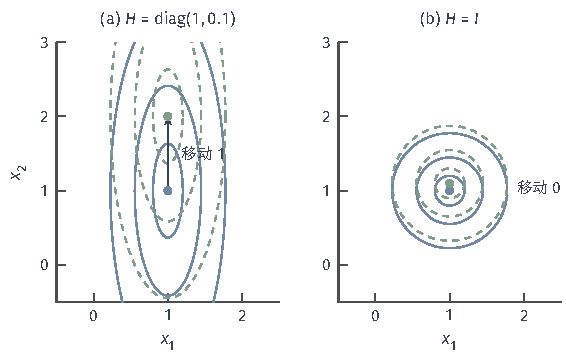
\includegraphics[width=95.8mm]{figures/03-optimization-evolution-and-signals/01-optimization/tikz/c3-sensitivity/figure.pdf}
  \caption{二次目标$f_{\bm b}(\bm x)=\tfrac12\bm x^\top\bm H\bm x-\bm b^\top\bm x$在数据改变前（蓝色实线）与改变后（绿色虚线）的等高线及最小点，两图中$b_2$都增加$0.1$。(a) $\bm H=\operatorname{diag}(1,0.1)$：$x_2$方向曲率只有$0.1$，最小点从$(1,1)$移到$(1,2)$，移动$1$。(b) $\bm H=\bm I$：最小点从$(1,1)$移到$(1,1.1)$，移动$0.1$。}
  \label{fig:opt-smooth-sensitivity}
\end{figure}

\paragraph{多解时先约定比较什么}
解不唯一时，“最优解怎样变化”需要先约定比较的对象。取$\bm H=\operatorname{diag}(1,0)$，它半正定而不正定。$\bm b=(1,0)^\top$时，$f_{\bm b}=\tfrac12x_1^2-x_1$，解集是整条直线$\{(1,s):s\in\mathbb R\}$；若约定选范数最小的解，得到$(1,0)^\top$。把数据改成$\bm b=(1,\epsilon)^\top$，$\epsilon\neq0$，目标多出一项$-\epsilon x_2$，沿$x_2$方向无下界，最优解根本不存在。无论$\epsilon$多小，解映射都从“一条直线”跳到“空集”。所以在多解问题中，不能不加约定就把最优解写成数据的单值连续函数：要么比较整个解集（例如用集合之间的距离），要么固定一个选解规则（例如最小范数），并分别检查这个规则下的解是否存在、是否连续。由数据选择函数时的选解问题在第~\ref{chap:opt-function-fitting}章展开。

\subsection{强凸目标的扰动界}
\label{sec:opt-smooth-strongly-convex-perturbation}

上面的例子提示，曲率的下界决定了解对线性扰动的敏感程度。下面把这一点写成一般结论。

\paragraph{线性扰动下的解变化}
第~\ref{chap:optimization}章的强凸一阶下界可以写成两个方向，再相加：对$\mu$强凸的可微函数$f$和任意$\bm x,\bm y$，
\[
  \begin{gathered}
  f(\bm y)\geq f(\bm x)+\langle\nabla f(\bm x),\bm y-\bm x\rangle+\frac\mu2\lVert\bm y-\bm x\rVert_2^2,\\
  f(\bm x)\geq f(\bm y)+\langle\nabla f(\bm y),\bm x-\bm y\rangle+\frac\mu2\lVert\bm x-\bm y\rVert_2^2 ,
  \end{gathered}
\]
相加得
\begin{equation}
\label{eq:opt-smooth-strong-monotone}
  \langle\nabla f(\bm x)-\nabla f(\bm y),\bm x-\bm y\rangle\geq\mu\lVert\bm x-\bm y\rVert_2^2 .
\end{equation}
这个性质称为梯度的\term{强单调性}（strong monotonicity）：梯度之差在位移方向上的投影，至少与位移的长度平方成正比。

\begin{theorem}[线性扰动下的解变化界]
\label{thm:opt-smooth-perturbation-bound}
设$f:\mathbb R^d\to\mathbb R$可微且$\mu$强凸（$\mu>0$），对$\bm b\in\mathbb R^d$令$f_{\bm b}(\bm x)=f(\bm x)-\langle\bm b,\bm x\rangle$。则每个$f_{\bm b}$有唯一最小点$\bm x_{\bm b}$，并且对任意$\bm b,\bm c$，
\[
  \lVert\bm x_{\bm b}-\bm x_{\bm c}\rVert_2\leq\frac1\mu\lVert\bm b-\bm c\rVert_2 .
\]
\end{theorem}

\begin{proof}
减去线性函数不改变强凸常数，所以$f_{\bm b}$仍是$\mu$强凸的；由第~\ref{chap:optimization}章，有限维上可微的强凸函数存在唯一最小点，且最小点处梯度为零，即$\nabla f(\bm x_{\bm b})=\bm b$，$\nabla f(\bm x_{\bm c})=\bm c$。代入式~\eqref{eq:opt-smooth-strong-monotone}，再用Cauchy--Schwarz不等式：
\[
  \mu\lVert\bm x_{\bm b}-\bm x_{\bm c}\rVert_2^2\leq\langle\bm b-\bm c,\bm x_{\bm b}-\bm x_{\bm c}\rangle\leq\lVert\bm b-\bm c\rVert_2\lVert\bm x_{\bm b}-\bm x_{\bm c}\rVert_2 .
\]
$\bm x_{\bm b}\neq\bm x_{\bm c}$时两边除以$\lVert\bm x_{\bm b}-\bm x_{\bm c}\rVert_2$即得结论，相等时结论显然。
\end{proof}

界中的$1/\mu$是精确的。对二次目标$\bm x_{\bm b}=\bm H^{-1}\bm b$，扰动沿最小特征值$\mu$的特征方向时，解的变化恰为$\lVert\delta\bm b\rVert_2/\mu$；图~\ref{fig:opt-smooth-sensitivity}(a)正是这种情形，$\mu=0.1$，扰动$0.1$造成移动$1$。解唯一并不意味着解稳定：$\mu$很小时，唯一的解可以对数据极为敏感。

\paragraph{绝对放大与条件数}
$1/\mu$度量的是绝对放大：数据改变一个单位，解最多改变多少个单位。它依赖于数据的尺度。另一种度量是相对的：对正定二次目标，由$\lVert\bm b\rVert_2\leq\lambda_{\max}\lVert\bm x_{\bm b}\rVert_2$与$\lVert\delta\bm x\rVert_2\leq\lVert\delta\bm b\rVert_2/\lambda_{\min}$，
\[
  \frac{\lVert\delta\bm x\rVert_2}{\lVert\bm x_{\bm b}\rVert_2}\leq\kappa(\bm H)\,\frac{\lVert\delta\bm b\rVert_2}{\lVert\bm b\rVert_2},\qquad\kappa(\bm H)=\frac{\lambda_{\max}(\bm H)}{\lambda_{\min}(\bm H)} .
\]
\term{条件数}（condition number）$\kappa$度量相对误差的放大，与整体尺度无关。两种度量回答不同的问题：$\bm H=\epsilon\bm I$的条件数是$1$，相对误差不放大，绝对误差却放大$1/\epsilon$倍。线性方程的条件数及其误差分析，参见本章前面引用的卷一“谱和奇异值”章。

\paragraph{问题的病态与算法的稳定}
本节的敏感性与上一节的误差传播是两件事。上一节的传播系数$q$描述算法在同一个问题上怎样处理执行误差，它取决于步长等算法选择；本节的$1/\mu$与$\kappa$描述问题本身，与算法无关。在病态问题上，再精确的算法也只能给出带误差数据所对应的最优解，提高求解精度不能消除问题自身的病态；要减小这部分误差，只能改善数据，或者改变问题本身，例如加入正则化项，这在第~\ref{chap:opt-function-fitting}章讨论。还要注意，本节只处理无约束目标中线性项的扰动。约束边界随数据移动、起作用的约束集合发生切换时，解可能不连续地跳动，需要第~\ref{chap:constrained-optimization}章的乘子与对偶工具来分析。
